\documentclass[lang=cn,a4paper]{elegantpaper}

\title{基于大数据的老旧小区加装电梯出资分摊方案的数学建模研究}
\author{作者:陶理 \and 指导老师:季鑫}
\institute{上海市实验学校}
\date{\zhtoday}

\usepackage{url,appendix,float,graphicx}

\begin{document}

    \maketitle
    
    \begin{abstract}
        \keywords{老旧小区加装电梯,数学建模,大数据}
    \end{abstract}

    \section{引言}

    \subsection{背景介绍}

    随着中国城市化进程的不断推进,各地的大规模城市建设正如火如荼地进行。与此同时,各大城市中许多上世纪90年代建造的老旧居民小区已不适应现代的生活需求,其升级改造势在必行。并且,老旧小区在各大城市中的占比很高\cite{research.ke},对于城市的美观有负面影响。所以对于老旧小区的改造势在必行。

    \begin{figure}[H]
        \centering
        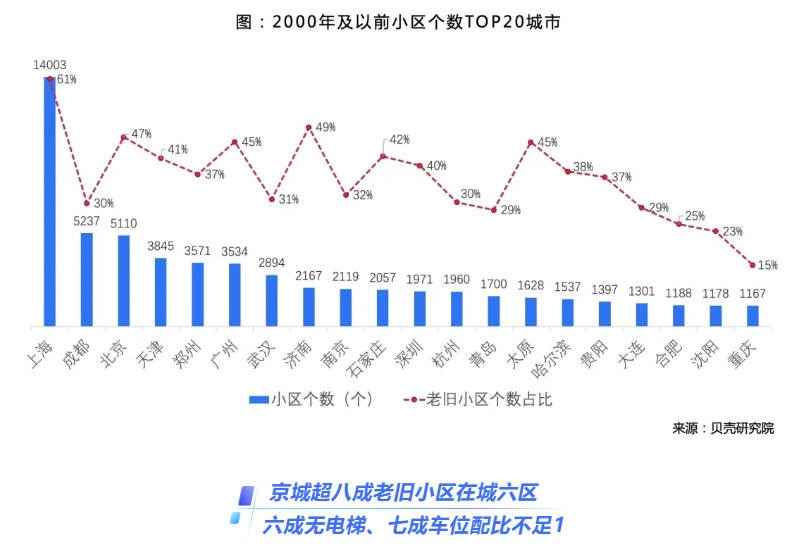
\includegraphics[scale=0.3]{number of old.png}
    \end{figure}
    老旧小区改造中的重要一项是为低层建筑(主要为六层楼房)加装电梯。电梯的安装将极大地方便居民出行和物流服务,特别是在提升深度老龄化群体的生活品质方面具有重要的意义。
    
    在此过程中涉及到一个关键问题是居民的出资分摊方案。除政府补助部分之外,目前一般的方案是按照楼层高度以简单的正比例函数的形式进行分摊,即$C=\dfrac{kL}{N}$\footnote{$C$表示每一户需要分摊的金额;$k$表示分摊系数;\\$L$表示楼层数;$N$表示每层楼的户数}。然而,这一简单方案难以准确反映不同楼层对于加装电梯的实际需求以及后续相关的商业增值。一般来说,较高楼层(5、6楼)原本由于上下楼不方便价值并不显著,但是加装电梯后,高楼层采光等优势愈发明显;低楼层对于电梯的需求本来不大,而且加装电梯后采光的劣势增加。所以各楼户的增值并非与楼层成正比,原本的分摊方案并不科学经济。
    
    \subsection{研究目的}
    提出一个数学模型,形如$f(a_1,a_2,\dots,a_n)=k$,将地段、楼层、居住者年龄/健康情况等各方面影响因素均定性处理作为变量,输出该楼栋加装电梯适宜的分摊比例。

    模型旨在打破常规的正比例函数式分摊比例,用大数据说明事实,更加科学理性地体现各个楼层之间的利益变化量,用以更加公平地调和不同楼层之间利益的变化导致的冲突和不愉快。
    \subsection{研究方法}

    \subsubsection{问卷调查法}
    通过问卷\footnote{见附录A、B},调查上海市部分已改造老旧小区的信息和数据:地段信息(如是否靠近地铁/是否为学区房等)、加装电梯前后不同楼层的户主对于自己房产的价值估计、不同楼层对于加装电梯的态度以及支持或者反对的原因。

    问卷调查有着高效率、调查范围广的优点,可以在较短时间内收集到较多的统一特征的数据。但是问卷调查的缺点也十分明显,如果受调查人员范围过广,导致调查结果不能充分反映所调研方面的数据;或者受调查人员填写问卷时十分草率,导致调查数据没有参考意义。因此,本次调查针对上海市已改造老旧小区的户主进行调查,通过联系居委会分发问卷以及在微信朋友圈中转发传播,尽量减少问卷受到受调查者主观情感意愿的影响。

    \subsubsection{建模法}
    通过建立模型的方式对于问卷所收集的数据进行数学分析。建立数学模型的方法能够定量地研究数据之间的关系,从而理性地根据给定的新数据预测新的结果。借助机器学习或者统计图表及其他统计学方法,可以较为简单地发现各种数据之间的联系。但是需要注意防止出现因果关系颠倒,避免研究不相关的两个变量之间的关系。

    \section*{致谢}
    在论文完成之际,我想要感谢我的班主任,也是我的指导老师季鑫:季老师,他在问卷调查、统计分析、小论文撰写等方面都给予了很大的帮助,凭借自己的经验也对于我小论文后期的完善有很多的帮助。同时感谢我的同班同学们,他们十分热心地转发了我的问卷,我才得以有比较完善的数据体系。特别感谢卢薏安同学,她在我的小论文撰写期间提供了许多思路和建议,对于论文的排版和美化也提出了许多自己的见解和建议。
    
    \clearpage

    \bibliography{reference}
    
    \clearpage
    
    \section*{附录}
    \appendix

    \section{关于老旧小区加装电梯的数据和户主态度的调研}

\end{document}